\documentclass{beamer}
\usetheme{metropolis} % Use metropolis theme
\title{Assignment 3 Presentation}
\date{\today}
\author{Ravi Kumar | Vighnesh J R | Shreyas N B | Mayank Ghritlahre}
\institute{AE667 Rotary Wing Aerodynamics - Group 1}
\begin{document}
\maketitle


\begin{frame}{Team Contribution}
    \begin{table}
        \centering
        \begin{tabular}{|c|c|c|c|} \hline 
            \textbf{Roll Number} & \textbf{Name} & \textbf{Contribution} & \textbf{Remarks}\\ \hline 
            210010052 & Ravi Kumar & 5 & Code \\
            210010073 & Vighnesh J R & 5 & Theory\\ 
            210010061 & Shreyas N B & 5 & Code, Slides\\ 
            210010040 & Mayank Ghritlahre & 5 & Slides\\ \hline
        \end{tabular}
    \end{table}
\end{frame}

  

\begin{frame}{Assumptions and Data}
\textbf{Physics Assumptions/Data}
\begin{itemize}
  \item The flight simulator updates parameters, forces, and moments every second.
  \item Gravity remains constant with altitude ($g = 9.81 \ m/s^2 \ \widehat{Z}_{hel}$).
\end{itemize}

\textbf{Environmental Assumptions/Data}
\begin{itemize}
  \item We apply the ISA (International Standard Atmosphere) model, linearly interpolating values based on helicopter altitude.
\end{itemize}

\textbf{Flight Condition Assumptions/Data}
\begin{itemize}
  \item The helicopter is in level flight at a constant altitude with no wind.
\end{itemize}
\end{frame}

\begin{frame}{Vehicle and Flight Condition Assumptions}
\textbf{Vehicle Assumptions/Data}
\begin{itemize}
  \item Inviscid, compressible $\left(\frac{1}{\sqrt{1-M_{\infty}^2}}\right)$ flow is assumed for the rotors.
  \item The engine is Turbotech, using Jet A1 fuel with a calorific value of $43.124 \ MJ/kg$ (based on a given data model).
  \item NACA0012 C$_{L}$ vs $\alpha$ $(0-360^\circ)$ data was obatined using WebPlotDigitizer from a given graph.
  \item Mass of vehicle is $50$ kg fuel, $50$ kg payload and $100$ kg structural weight.
\end{itemize}
\end{frame}

%
% %%%%%%%%%%%%%%%%%%%%%%%%%%%%%%%%%
\begin{frame}{Theoretical Reformulations}
  \textbf{Defining blade element Geometrically}
  \begin{figure}
      \centering
      \includegraphics[width=0.7\linewidth]{../images/Schematics.jpg}
      \caption{Visualisation of Airfoil plane and Blade plane}
      \label{fig: Schematics}
  \end{figure}
\end{frame}
\begin{frame}{Theoretical Reformulations}
    \textbf{Significance of Geometric approach}
    \begin{itemize}
        \item Every blade is given a blade plane normal $\hat{n}(\psi,\beta)$ and airfoil plane normal $\hat{r}(\psi,\beta)$ (towards the hub).
        \item The location of the blade is given by azimuth position $\psi$ and coning angle $\beta$
        \item Local relative velocity field projected onto the airfoil plane for sectional lift and drag computations as in figure 
        \ref{fig: Schematics}
        \item Aerodynamic force resolved along $\hat{n}$ and $\hat{n}\times\hat{r}$ as $dT$ and $dF_{\tau}$
        \item Airfoil pitch $\theta$ defined w.r.t blade plane
    \end{itemize}
\end{frame}
\begin{frame}{Theoretical Reformulations}
    \textbf{Vectors defined in hub frame}
    \begin{columns}[T] % align columns to the top
        % First column for the image
        \begin{column}{0.5\textwidth}
            \begin{figure}
                \centering
                \includegraphics[width=0.8\linewidth]{../images/Vectors.png}
                %\caption{Enter Caption}
                %\label{fig:enter-label}
            \end{figure}
        \end{column}
        
        % Second column for the text
        \begin{column}{0.5\textwidth}
            \begin{itemize}
                \item Figure given hub frame
                \item Blade normal given by
                $$
                \hat{n}(\psi,\beta) = \begin{bmatrix}
                    \sin(\beta)\cos(\psi) \\
                    \sin(\beta)\sin(\psi) \\
                    \cos(\beta)
                \end{bmatrix}
                $$
                \item Airfoil Plane normal given by 
                $$
                \hat{r}(\psi,\beta) = \begin{bmatrix}
                    \cos(\beta)\cos(\psi) \\
                    \cos(\beta)\sin(\psi) \\
                    -\sin(\beta)
                \end{bmatrix}
                $$
            \end{itemize}
        \end{column}
    \end{columns}
\end{frame}
\begin{frame}{Aerodynamics Modelling}
    Assume ambient velocity field $\vec{V}(r,\psi,z)$ over the rotor disk. The aerodynamic loads on a blade depends on the velocity faced by it projected onto the blade plane.
    \begin{figure}
        \centering
        \includegraphics[width=0.7\linewidth]{../images/Projection.png}
        \caption{Projection of velocity}
    \end{figure}
\end{frame}
\begin{frame}{Aerodynamics Modelling}
   The velocity relative to rotating blade is given by 
   \begin{equation*}
\vec{V}_{rel} = \vec{V} + \Omega r (\hat{n} \times \hat{r})
   \end{equation*}
   where $\Omega = \dot{\psi}$ and its projecting onto the airfoil plane is
   \begin{equation*}
       \vec{V}_{proj} = \vec{V}_{rel} - \hat{r}(\vec{V}_{rel}\cdot \hat{r})
   \end{equation*}
   Hence geometrically, the angle of attack faced by the airfoil is  
   \begin{equation*}
       \alpha = \theta + \underbrace{\tan^{-1}\left(\frac{\vec{V}_{proj}\cdot \hat{n}}{\vec{V}_{proj}\cdot (\hat{n}\times \hat{r})}\right)}_{ = - \phi}
   \end{equation*}
   Furthermore by neglecting the 3d flow effects, we compute the aerodynamic coefficients and integrate the forces and moments.
\end{frame}
\begin{frame}{Blade Flapping}
    For a given flow field and blade location $\beta,\psi$ of a blade, we can compute the hinge moment acting it given by
    $$M_{\text{H}}(\beta,\psi) =\int_{R_{root}}^{R_{tip}}(\vec{F}_{\text{aero}}\cdot \hat{n}) r dr$$
    Where $\vec{F}_{\text{aero}}$ is the aerodynamic load on the blade. This moment is counteracted by the torque due to centrifugal forces given by $M_{c}(\beta) = \int r^2 \Omega^2 \cos^2(\beta)\sin(\beta)\mathbf{dm}$. This results in the blade flapping being stabilised at an equilibrium $\beta_{eq}(\psi)$  which is a solution of $M_H(\beta,\psi) - M_c(\beta) =0$, at a given azimuthal location. 
\end{frame}
\begin{frame}{Computation of Induced Velocity Field}
    The total velocity field inclusive of induced velocity field is computed iteratively for a main rotor setup as follows.
    \begin{itemize}
        \item Compute thrust with a nominal guess for induced inflow ratio.
        \item From thrust coefficient, compute the Glauert induced inflow ratio $\lambda_{i,G}$
        \item Construct the spatially varying induced velocity field and append it to the total velocity field (with learning rate)
        \item Iterate until thrust converges.
    \end{itemize}
\end{frame}
%%%%%%%%%%%%%%%%%%%%%%%%%%%%%%%%%%
%

\begin{frame}{Algorithm/Logic Flow Diagrams: mission.py}
    \begin{figure}
      \centering
      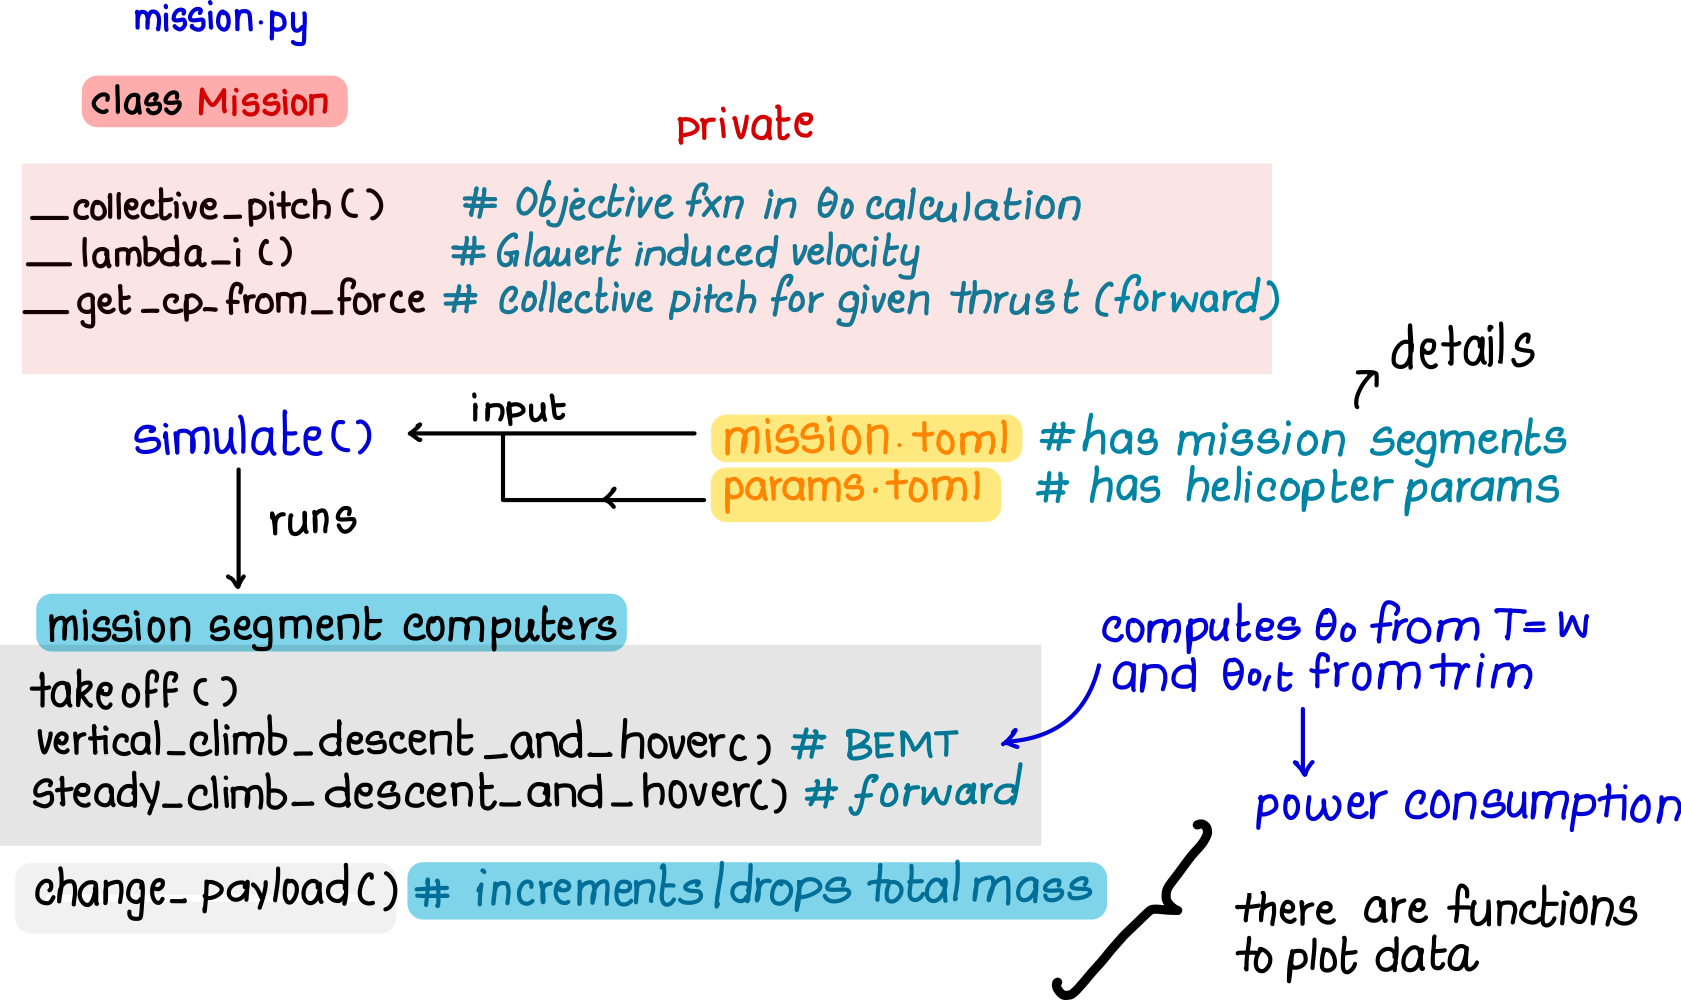
\includegraphics[width=\linewidth]{../images/mission.jpeg}
    \end{figure}
\end{frame}

\begin{frame}{Algorithm/Logic Flow Diagrams: mission.py}
    \begin{enumerate}
      \item The mission profile is provided through $\texttt{mission\_A.toml}, \texttt{mission\_B.toml}$, etc., files which contains the rates and distances for each individual segment.
      \item The script accounts for switching between forward flight (Glauert model) and hover (BEMT model) based on the mission profile, and also uses a dynamic time scale.
      \item The script calculates the gross weight, fuel consumption, fuel burn rate, altitude, power, speed, climb rate, and distance covered at each time interval.
    \end{enumerate}
\end{frame}

\begin{frame}{Algorithm/Logic Flow Diagrams: Mission computer}

  \begin{figure}
    \centering
    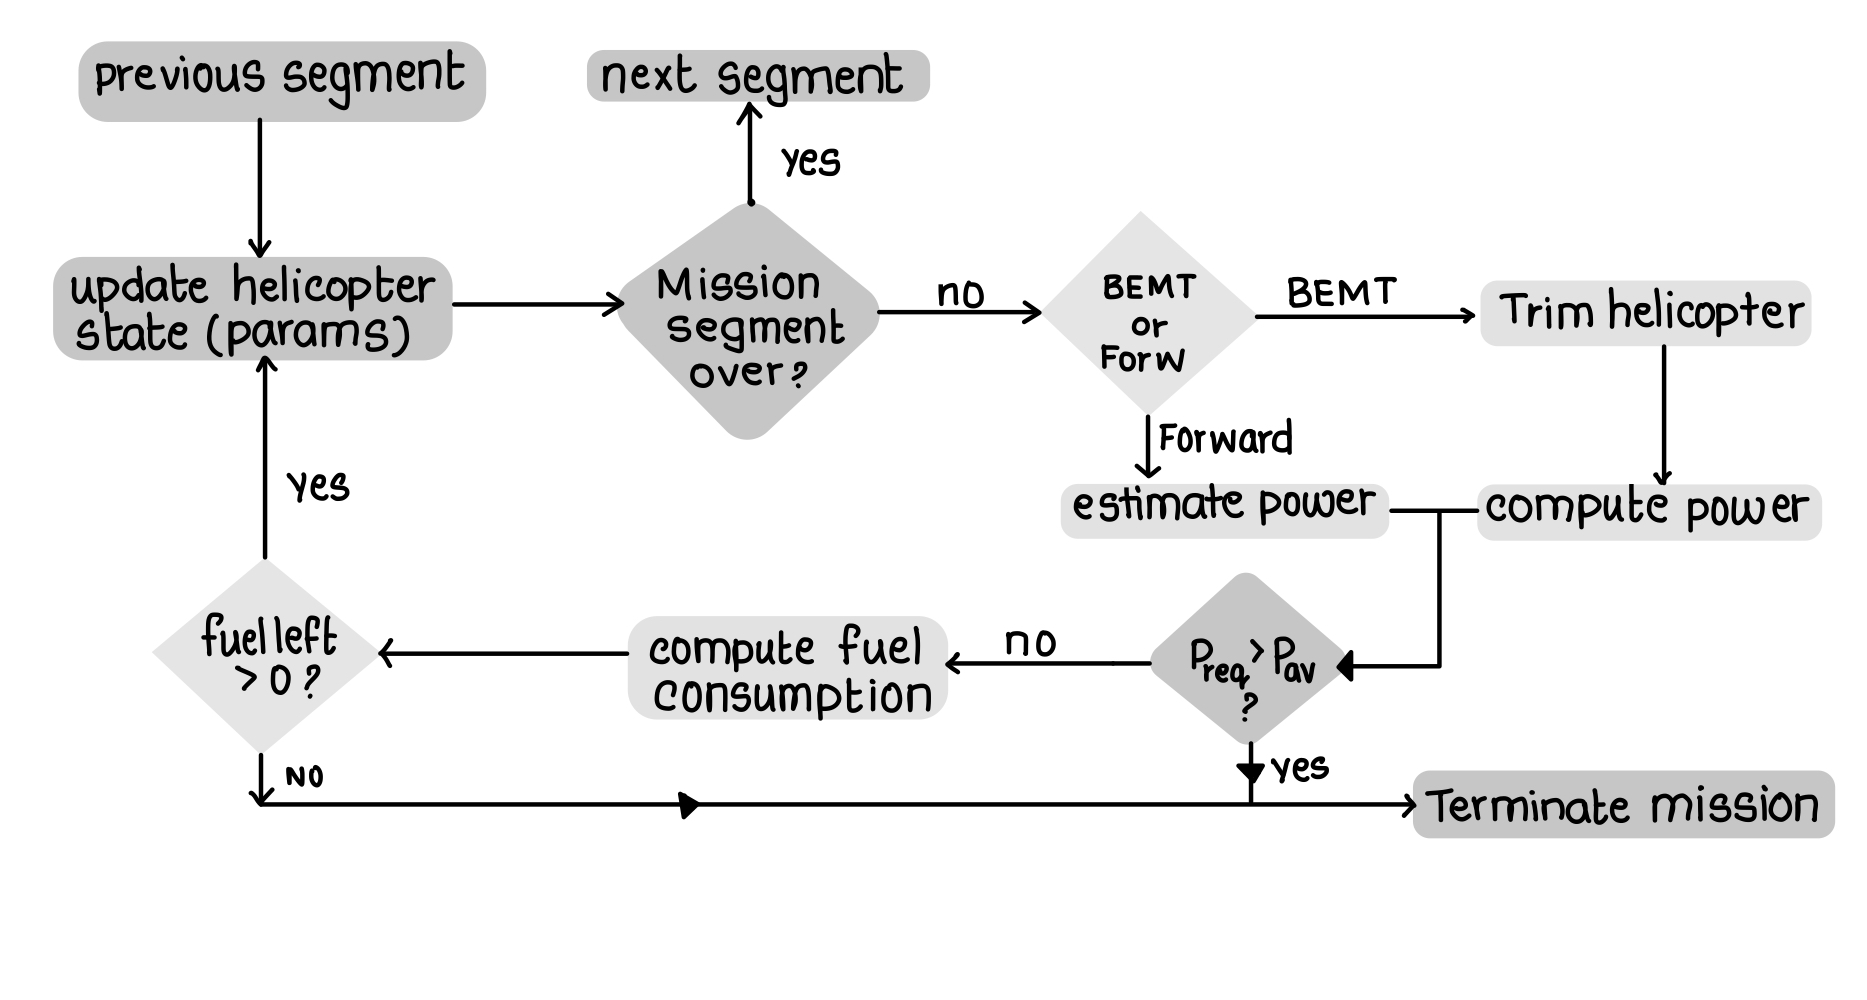
\includegraphics[width=\linewidth]{../images/mission_computer.jpeg}
  \end{figure}

\end{frame}

\begin{frame}{Algorithm/Logic Flow Diagrams: helicopter.py}
    This file combines dynamics from the two rotors, two stabilizers and the fuselage. It is initialized with a \texttt{params.toml} file as shown, and creates 2 \texttt{RotorBlade} objects for the main and tail rotors, and 2 \texttt{Wing} objects for the horizontal and vertical stabilizers.
    
    Control inputs are fed into these objects, and we use their functions described earlier to calculate the forces, moments, power etc.

    Almost all the quantities are in a vector form, so we just use vector algebra to sum them up and get the net quantities, which are then printed in a neat format to ease manual trimming (done through running \texttt{python helicopter.py}).
\end{frame}

\begin{frame}{Algorithm/Logic Flow Diagrams: helicopter.py}
    The \texttt{Wing} object is used to initialize the horizontal and vertical stabilizers using the design parameters given. We calculate the net lift and drag by using the net velocity over each and add it to the net force and moment.

    This is done by accounting for the wake of the main rotor flowing over the stabilizers, and we obtain this wake depending on the angle of attack at each radially discrete point on the TPP. If the wake is not able to reach the stabilizer at any point, then $V_{\infty}$ is used instead.

    A visualization of this is shown in the next slide.
\end{frame}

\begin{frame}{Algorithm/Logic Flow Diagrams: helicopter.py}
  
  \begin{figure}
    \centering
    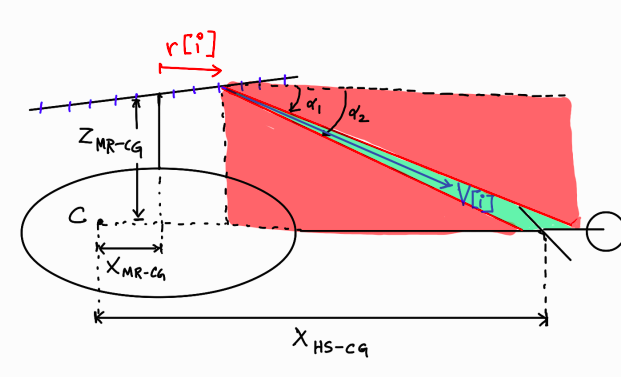
\includegraphics[width=0.7\linewidth]{../images/stab-wake.png}
    \caption{Main rotor wake on stabilizers}
  \end{figure}

  Hence, we only consider the wake of such elements which flow over the stabilizers (green region) by accounting for the angle of attack at each point on the TPP, i.e., $\alpha_1 \leq \alpha[i] \leq \alpha_2$.
\end{frame}

\begin{frame}{Algorithm/Logic Flow Diagrams: trim\_curve.ipynb}
      Here we use the simplified power coefficient expression to estimate the main and tail rotor power at each time interval in various flight conditions. 

      \[
        C_p = \kappa C_T \lambda_i + \dfrac{1}{2}\dfrac{f}{A}\mu^3 + \dfrac{\sigma C_{d0}}{8}[1+4.6\mu^2]
      \]

      During the mission planner test, we will have access to only approximate solutions for $C_T$, $\mu$, $\lambda_i$ and $\alpha_\text{TPP}$. So, we trim the helicopter \textbf{but} use the below approximate expressions to fit the power coefficient curve.
      
      \[
        C_T = \dfrac{\sqrt{W^2+D^2}}{\rho_\infty (\Omega R)^2} \quad \alpha_\text{TPP} = \tan^{-1}{\dfrac{D}{W}} \quad \mu  = \dfrac{V_\infty\cos{\alpha_\text{TPP}}}{\Omega R}
      \]
\end{frame}

\begin{frame}{Algorithm/Logic Flow Diagrams: trim\_curve.ipynb}
  $\lambda_i$ needs to be solved iteratively and is dependent on $\mu, C_T, \alpha_\text{TPP}$. 
  We do this by defining an objective function \texttt{\_\_lambda\_i} which takes $\mu, C_T, \alpha_\text{TPP}$ and uses \texttt{fsolve} to solve for $\lambda_i$ inside the \texttt{cal\_median\_forward\_flight\_params} function.

  Also, we fit only the main rotor power curve and then calculate the ratio between the main and tail rotor power  and fit a straight line to it to get the tail rotor power as a function of main rotor power. This was done as we are not fully convinced of fitting the curve for tail rotor after neglecting the fuselage drag term.
\end{frame}

\begin{frame}{Algorithm/Logic Flow Diagrams: trim\_curve.ipynb}
  \begin{figure}[h!]
    \centering
    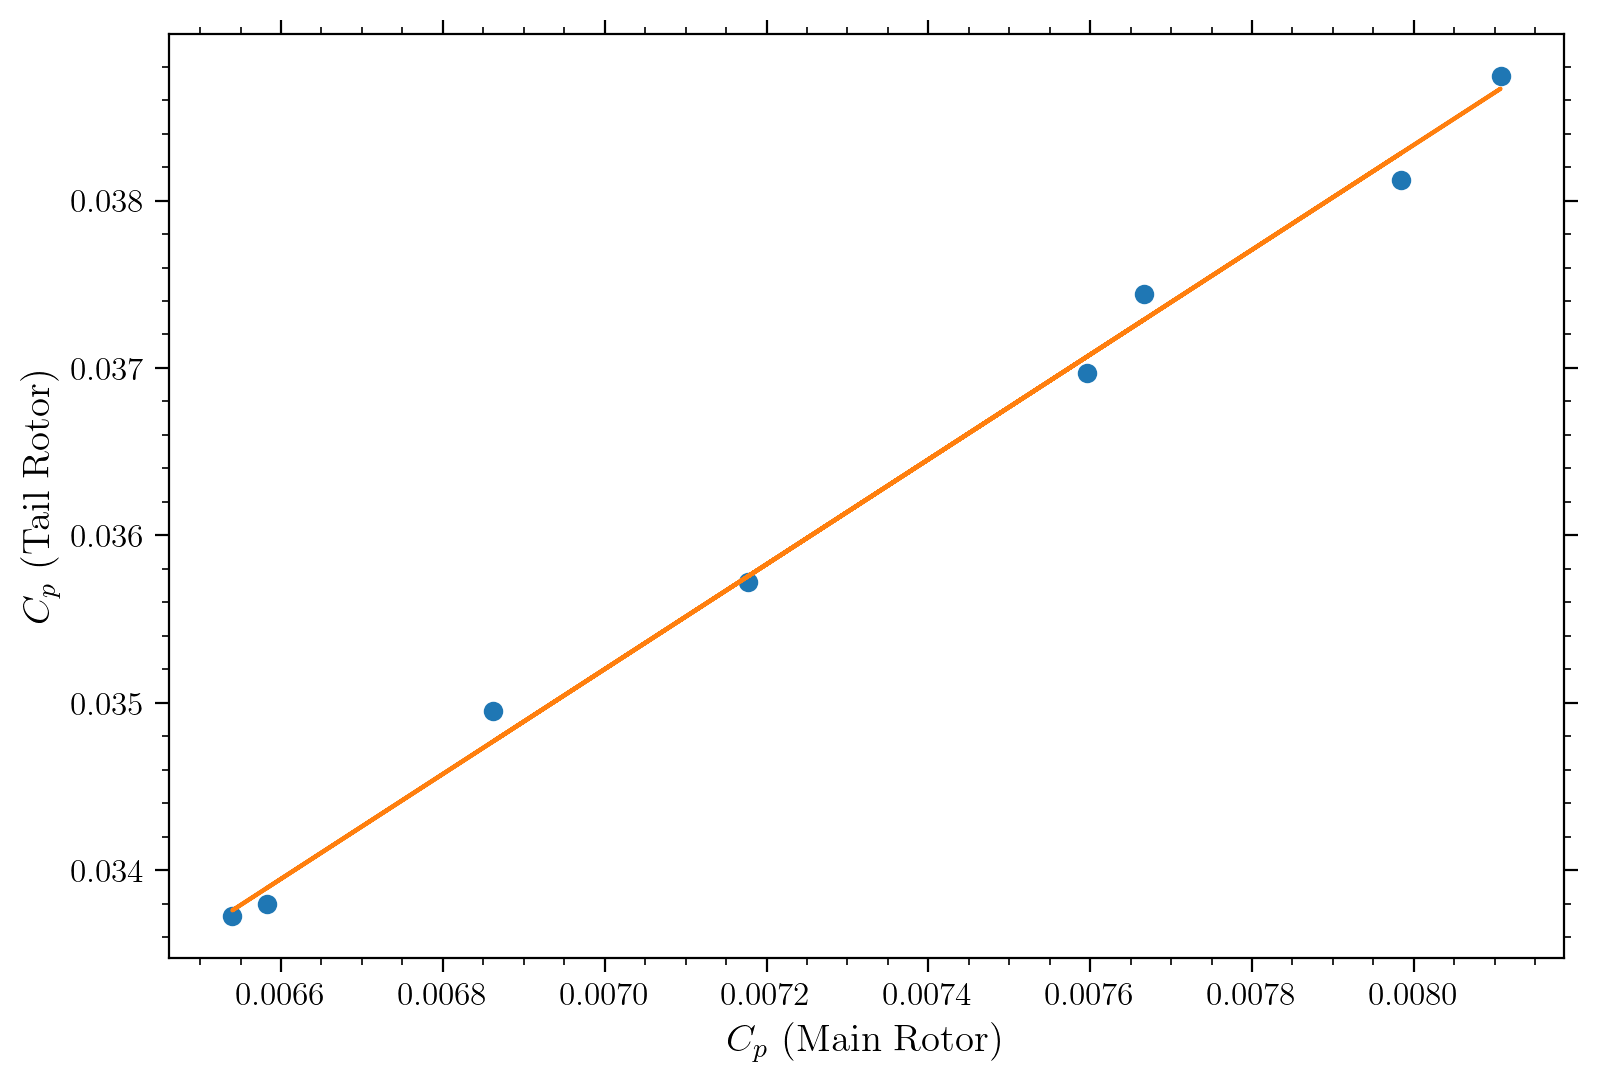
\includegraphics[width=0.8\linewidth]{../images/cp_tail_rotor_vs_cp_main_rotor.png}
    \caption{Tail rotor power vs Main rotor power}
  \end{figure}
\end{frame}

\begin{frame}{Algorithm/Logic Flow Diagrams: trim\_curve.ipynb}
  \begin{figure}[h!]
    \centering
    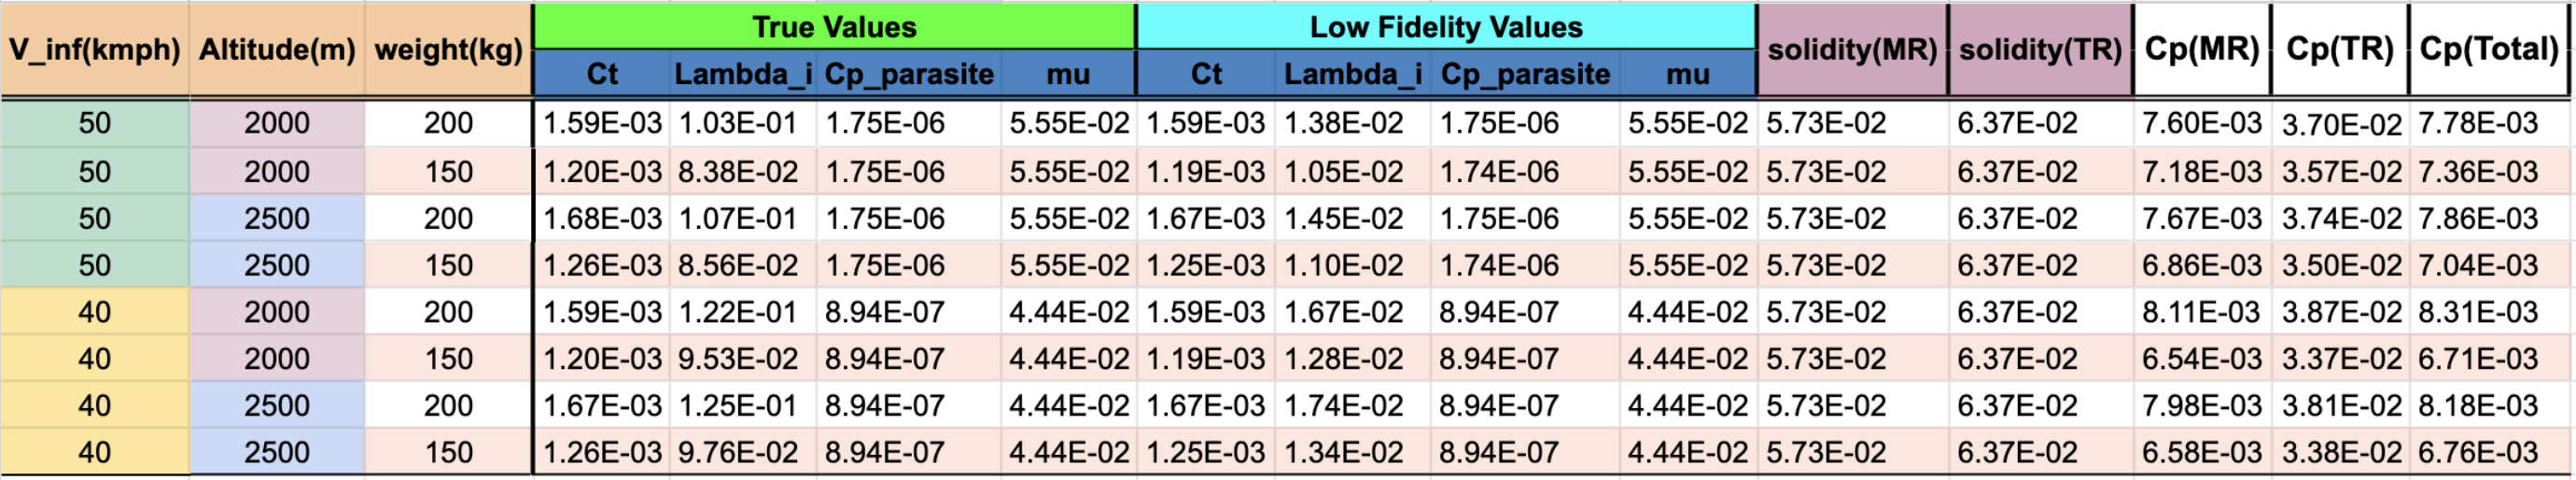
\includegraphics[width=\linewidth]{../images/trim_table.png}
    \caption{Table of altitudes, gross weights and trim settings}
  \end{figure}
  The complete values can be found at \texttt{data/trim\_curve.csv}.
  We get the following values after fitting:
  \[
    \kappa \rightarrow 25.85 \quad C_{d0} \rightarrow 0.48 \quad 4.6 \rightarrow 139.52
  \]
  \[
    C_{P_\text{tail rotor}} = 3.13 C_{P_\text{main rotor}} + 1.33 \times 10^{-2}
  \]
\end{frame}

  \begin{frame}{Algorithm/Logic Flow Diagrams: optimize\_mission.py}

    This code simply runs the individual mission profile A in a loop with varying maximum altitudes in order to determine the maximum altitude at which the mission can be completed. This is done to ease some load on manually finding this altitude.

  \end{frame}


\begin{frame}{Algorithm/Logic Flow Diagrams}
    \textbf{Note:}
    Please refer to the code files for further understanding and the functions' inputs/outputs, as there are various internal functions not shown in the diagrams. Each function has a docstring explaining its inputs and purpose. The variables are also named in a self-explanatory manner.

\end{frame}

\begin{frame}{Test Vehicle}
  The design parameters have been chosen same as in Assignment-2.
    \begin{center}
        $\alpha_\text{fuselage} = 1^\circ$
        \end{center}
        \begin{table}
            \centering
            \begin{tabular}{|c|c|c|}
            \hline
                \textbf{Parameter} & \textbf{Main Rotor} & \textbf{Tail Rotor} \\ \hline
                 Airfoil & NACA 0012 & NACA 0012\\ \hline
                 Rotor radius (m)& 2.5 & 0.5\\ \hline
                 Rotor speed (rad/s)& 100 & 400 \\ \hline
                 Number of blades & 3 & 2\\ \hline
                 Root cutout (m) & 0.1  & 0.025\\ \hline
                 Chord length variation & 0.2 $\to$ 0.10 & 0.05 $\to$ 0.05\\ \hline
                 Twist variation (m$^{-1}$) & $0^\circ$ & $0^\circ$\\ \hline
                 \hline
            \end{tabular}
        \end{table} 
\end{frame}

\begin{frame}{Test Vehicle}

  \begin{table}
    \centering
    \begin{tabular}{|c|c|c|}
      \hline
      \textbf{Parameter} & \textbf{Horizontal Stabilizer} & \textbf{Vertical Stabilizer} \\ \hline
      Airfoil & NACA 0012 & NACA 0012\\ \hline
      Span (m) & 0.8 & 0.7\\ \hline
      Chord (m) & 0.2 & 0.3\\ \hline
    \end{tabular}
  \end{table}

\end{frame}

\begin{frame}{Test Vehicle}

  The distances of the stabilizers have been chosen differently from given parameters, so that it matches our Assignment 2 helicopter.

\begin{center}
    $X_{MR-CG}$ = 0m; $X_{TR-CG}$ = 4.75m
    
    $Z_{MR-CG}$ = 1.5m; $Z_{TR-CG}$ = 1m

    $X_{HS-CG}$ = 3.5m; $X_{VS-CG}$ = 4.75m

    $Z_{HS-CG}$ = 1m; $Z_{VS-CG}$ = 1m
\end{center}

\begin{figure}
    \centering
    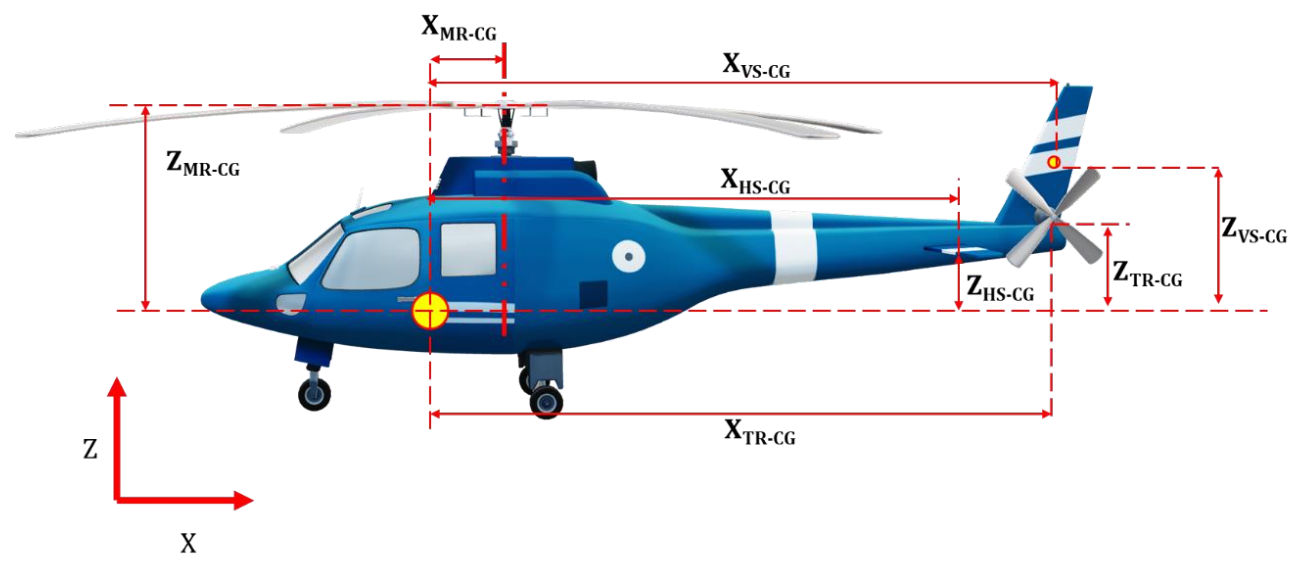
\includegraphics[width=0.75\linewidth]{../images/test_helicopter.png}
    \caption{Test Vehicle}
\end{figure}
\end{frame}

\begin{frame}{Trim Settings}
    \textbf{Trim}
    
  For a 50 km/h level flight at 2000 m AMSL with $\alpha_\text{fuselage} = 1^\circ$ on addition of stabilizers:
  \begin{table}[ht]
      \centering
      \renewcommand{\arraystretch}{1.4} % Increase the row height
      \setlength{\tabcolsep}{12pt} % Adjust column separation
      \begin{tabular}{|c|c|c|c|}
          \hline
          &(degrees)  & &(N or N-m, Vehicle)  \\
          \hline
          \textbf{$\theta_{o,m}$} & 2.267 & \textbf{$F_X$} & -0.008 \\ 
          \hline
          \textbf{$\theta_{1c}$} & 1.55 & \textbf{$F_Y$} & 25.05 \\ 
          \hline
          \textbf{$\theta_{1s}$} & 2.62 & \textbf{$F_Z$} & 0.56 \\ 
          \hline
          \textbf{$\theta_{o,t}$} & 2.6 & \textbf{$M_X$} & 12.46 \\ 
          \hline
          \textbf{$\alpha_{TPP}$} & 1.167 & \textbf{$M_Y$} & 16.01 \\ 
          \hline
          \textbf{$\beta_{o}$} & 0.3 & \textbf{$M_Z$} & -0.78 \\ 
          \hline
      \end{tabular}
      \caption{Trim Settings}
      \label{tab:trim_settings}
  \end{table}
  
  \end{frame}




\begin{frame}{Mission planner test}
    \textbf{Mission A: Successful payload drop mission}

    We assume the following rates and distances for this mission:

    \begin{table}
        \centering
        \begin{tabular}{|c|c|} \hline 
            Vertical climb & Climb velocity = 1m/s \\ \hline 
            Steady climb & \begin{tabular}{c}Climb velocity = 4 m/s \\ Forward Velocity = 9 m/s \end{tabular} \\ \hline 
            Level Flight &  \begin{tabular}{c}Forward Velocity = 14m/s \\ Distance = 5 km \end{tabular}\\ \hline
            Steady descent & \begin{tabular}{c}Climb velocity = -0.5m/s \\ Forward Velocity = 9 m/s \end{tabular}\\ \hline
            Vertical descent & Climb velocity = -0.5m/s \\ \hline
        \end{tabular}
    \end{table}

\end{frame}

\begin{frame}{Mission planner test: Mission A plots}
  \begin{figure}
    \centering
    \includegraphics[width=0.9\linewidth]{../images/mission_A/Gross_Weight.png}
    \caption{Gross Weight vs Time}
  \end{figure}
\end{frame}

\begin{frame}{Mission planner test: Mission A plots}
  \begin{figure}
    \centering
    \includegraphics[width=0.9\linewidth]{../images/mission_A/Fuel.png}
    \caption{Fuel vs Time}
  \end{figure}
\end{frame}

\begin{frame}{Mission planner test: Mission A plots}
  \begin{figure}
    \centering
    \includegraphics[width=0.9\linewidth]{../images/mission_A/Fuel_Burn_Rate.png}
    \caption{Fuel Burn Rate vs Time}
  \end{figure}
\end{frame}

\begin{frame}{Mission planner test: Mission A plots}
  \begin{figure}
    \centering
    \includegraphics[width=0.9\linewidth]{../images/mission_A/Altitude.png}
    \caption{Altitude vs Time}
  \end{figure}

\end{frame}

\begin{frame}{Mission planner test: Mission A plots}
  \begin{figure}
    \centering
    \includegraphics[width=0.9\linewidth]{../images/mission_A/Power.png}
    \caption{Power vs Time}
  \end{figure}
\end{frame}

\begin{frame}{Mission planner test: Mission A plots}
  \begin{figure}
    \centering
    \includegraphics[width=0.9\linewidth]{../images/mission_A/Speed.png}
    \caption{Speed vs Time}
  \end{figure}
\end{frame}

\begin{frame}{Mission planner test: Mission A plots}
  \begin{figure}
    \centering
    \includegraphics[width=0.9\linewidth]{../images/mission_A/Climb_Rate.png}
    \caption{Climb Rate vs Time}
  \end{figure}
\end{frame}

\begin{frame}{Mission planner test: Mission A plots}
  \begin{figure}
    \centering
    \includegraphics[width=0.9\linewidth]{../images/mission_A/Distance_Covered.png}
    \caption{Distance Covered vs Time}
  \end{figure}
\end{frame}


\begin{frame}{Mission planner test}
  \textbf{Mission B: Successful payload pickup mission}

  We assume all the same rates and distances as in Mission A, except the fact that takeoff payload is $0$ kg and payload is picked up instead of being dropped.

\end{frame}

\begin{frame}{Mission planner test: Mission B plots}
  \begin{figure}
    \centering
    \includegraphics[width=0.9\linewidth]{../images/mission_B/Gross_Weight.png}
    \caption{Gross Weight vs Time}
  \end{figure}
\end{frame}

\begin{frame}{Mission planner test: Mission B plots}
  \begin{figure}
    \centering
    \includegraphics[width=0.9\linewidth]{../images/mission_B/Fuel.png}
    \caption{Fuel vs Time}
  \end{figure}
\end{frame}

\begin{frame}{Mission planner test: Mission B plots}
  \begin{figure}
    \centering
    \includegraphics[width=0.9\linewidth]{../images/mission_B/Fuel_Burn_Rate.png}
    \caption{Fuel Burn Rate vs Time}
  \end{figure}
\end{frame}

\begin{frame}{Mission planner test: Mission B plots}
  \begin{figure}
    \centering
    \includegraphics[width=0.9\linewidth]{../images/mission_B/Altitude.png}
    \caption{Altitude vs Time}
  \end{figure}

\end{frame}

\begin{frame}{Mission planner test: Mission B plots}
  \begin{figure}
    \centering
    \includegraphics[width=0.9\linewidth]{../images/mission_B/Power.png}
    \caption{Power vs Time}
  \end{figure}
\end{frame}

\begin{frame}{Mission planner test: Mission B plots}
  \begin{figure}
    \centering
    \includegraphics[width=0.9\linewidth]{../images/mission_B/Speed.png}
    \caption{Speed vs Time}
  \end{figure}
\end{frame}

\begin{frame}{Mission planner test: Mission B plots}
  \begin{figure}
    \centering
    \includegraphics[width=0.9\linewidth]{../images/mission_B/Climb_Rate.png}
    \caption{Climb Rate vs Time}
  \end{figure}
\end{frame}

\begin{frame}{Mission planner test: Mission B plots}
  \begin{figure}
    \centering
    \includegraphics[width=0.9\linewidth]{../images/mission_B/Distance_Covered.png}
    \caption{Distance Covered vs Time}
  \end{figure}
\end{frame}

\begin{frame}{Mission planner test}
  \textbf{Mission C: Fuel limited unsuccessful payload pickup mission}

  We assume all the same rates as in Mission B. The distance covered in the level flight segment is increased to $520$ km. This results to fuel running out in the steady flight segment after picking up the payload.

\end{frame}

\begin{frame}{Mission planner test: Mission C plots}
  \begin{figure}
    \centering
    \includegraphics[width=0.9\linewidth]{../images/mission_C/Gross_Weight.png}
    \caption{Gross Weight vs Time}
  \end{figure}
\end{frame}

\begin{frame}{Mission planner test: Mission C plots}
  \begin{figure}
    \centering
    \includegraphics[width=0.9\linewidth]{../images/mission_C/Fuel.png}
    \caption{Fuel vs Time}
  \end{figure}
\end{frame}

\begin{frame}{Mission planner test: Mission C plots}
  \begin{figure}
    \centering
    \includegraphics[width=0.9\linewidth]{../images/mission_C/Fuel_Burn_Rate.png}
    \caption{Fuel Burn Rate vs Time}
  \end{figure}
\end{frame}

\begin{frame}{Mission planner test: Mission C plots}
  \begin{figure}
    \centering
    \includegraphics[width=0.9\linewidth]{../images/mission_C/Altitude.png}
    \caption{Altitude vs Time}
  \end{figure}

\end{frame}

\begin{frame}{Mission planner test: Mission C plots}
  \begin{figure}
    \centering
    \includegraphics[width=0.9\linewidth]{../images/mission_C/Power.png}
    \caption{Power vs Time}
  \end{figure}
\end{frame}

\begin{frame}{Mission planner test: Mission C plots}
  \begin{figure}
    \centering
    \includegraphics[width=0.9\linewidth]{../images/mission_C/Speed.png}
    \caption{Speed vs Time}
  \end{figure}
\end{frame}

\begin{frame}{Mission planner test: Mission C plots}
  \begin{figure}
    \centering
    \includegraphics[width=0.9\linewidth]{../images/mission_C/Climb_Rate.png}
    \caption{Climb Rate vs Time}
  \end{figure}
\end{frame}

\begin{frame}{Mission planner test: Mission C plots}
  \begin{figure}
    \centering
    \includegraphics[width=0.9\linewidth]{../images/mission_C/Distance_Covered.png}
    \caption{Distance Covered vs Time}
  \end{figure}
\end{frame}

\begin{frame}{Mission planner test}
  \textbf{Mission D: Power limited unsuccessful payload drop mission}

  We assume all the same rates and distances as in Mission A. The helicopter was made to takeoff and perform the mission segments at higher altitudes to check if the power limit is reached. The power limit was not reached even after fliying at 10 km, and going higher did not result in any changes as our ISA table (\texttt{data/isa.csv}) is limited to 10 km. 

  A probable cause for this could be that we had trimmed the helicopter in the 2000-2500 m range to obtain our best fit values of $\kappa, C_{d0}$ etc. So, the power calculations for higher altitudes wouldnt be accurate. This would require trimming repetitively at higher altitudes, which we did not do due how long it would take to trim each time.

\end{frame}

\begin{frame}{Mission planner test: Mission D plots}
  \begin{figure}
    \centering
    \includegraphics[width=0.9\linewidth]{../images/mission_D/Gross_Weight.png}
    \caption{Gross Weight vs Time}
  \end{figure}
\end{frame}

\begin{frame}{Mission planner test: Mission D plots}
  \begin{figure}
    \centering
    \includegraphics[width=0.9\linewidth]{../images/mission_D/Fuel.png}
    \caption{Fuel vs Time}
  \end{figure}
\end{frame}

\begin{frame}{Mission planner test: Mission D plots}
  \begin{figure}
    \centering
    \includegraphics[width=0.9\linewidth]{../images/mission_D/Fuel_Burn_Rate.png}
    \caption{Fuel Burn Rate vs Time}
  \end{figure}
\end{frame}

\begin{frame}{Mission planner test: Mission D plots}
  \begin{figure}
    \centering
    \includegraphics[width=0.9\linewidth]{../images/mission_D/Altitude.png}
    \caption{Altitude vs Time}
  \end{figure}

\end{frame}

\begin{frame}{Mission planner test: Mission D plots}
  \begin{figure}
    \centering
    \includegraphics[width=0.9\linewidth]{../images/mission_D/Power.png}
    \caption{Power vs Time}
  \end{figure}
\end{frame}

\begin{frame}{Mission planner test: Mission D plots}
  \begin{figure}
    \centering
    \includegraphics[width=0.9\linewidth]{../images/mission_D/Speed.png}
    \caption{Speed vs Time}
  \end{figure}
\end{frame}

\begin{frame}{Mission planner test: Mission D plots}
  \begin{figure}
    \centering
    \includegraphics[width=0.9\linewidth]{../images/mission_D/Climb_Rate.png}
    \caption{Climb Rate vs Time}
  \end{figure}
\end{frame}

\begin{frame}{Mission planner test: Mission D plots}
  \begin{figure}
    \centering
    \includegraphics[width=0.9\linewidth]{../images/mission_D/Distance_Covered.png}
    \caption{Distance Covered vs Time}
  \end{figure}
\end{frame}

\begin{frame}{Mission planner test - Observations}
  On analyzing the plots from various missions, we observe how the power varies with altitude, speed, and payload. We also see how the fuel consumption rate varies with time and how the gross weight changes with time. The distance covered by the helicopter is also plotted against time.
\end{frame}

\begin{frame}{Mission A Observations}
  \begin{enumerate}
    \item Sudden drop in gross weight observed due to payload drop
    \item Fuel burn rate decreases on payload drop (around 13 min)
    \item Fuel burn rate also decreases with time in each segment as net weight decreases.
    \item Power required increases with altitude, and decrease on payload drop.
    \item Distance covered (and fuel weight) is (are) linear with time and increasing (decreasing) as expected.
  \end{enumerate} 
\end{frame}

\begin{frame}{Mission B Observations}
  \begin{enumerate}
    \item Sudden spike in gross weight observed due to payload pickup.
    \item Fuel burn rate increases on payload pickup (around 13 min)
    \item Power required increases in hover segment, and also on payload pickup.
    \item One can also observe that average power required, and average fuel burn rate, before payload pickup is higher than after pickup.
  \end{enumerate}
\end{frame}

\begin{frame}{Mission C Observations}
  \begin{enumerate}
    \item Fuel runs out in the steady flight segment after picking up the payload (around 650 min).
    \item The plots may seem skewed due to the long duration of the level flight segment, but the trends are similar to Mission B.
    \item Abrupt changes are numerical issues due to timescale not being fine enough.
  \end{enumerate}
  
\end{frame}

\begin{frame}{Mission D Observations}
  \begin{enumerate}
    \item As discussed earlier, the power limit was not reached even at 10 km altitude.
    \item We observe that the power required peaks to 25 kW at the payload drop point (around 13 min), but the power available is still higher (at 35 kW). 
    \item The other trends are similar to Mission A, except for the limits, since the operation altitude is much higher.
  \end{enumerate}
  
\end{frame}

\begin{frame}{References}
 \begin{enumerate}
     \item Lecture Notes - AE 667 (Rotary Wing Aerodynamics) by Prof. Dhwanil Shukla
 \end{enumerate}
\end{frame}




\end{document}